\documentclass{article}
\usepackage{multido,graphicx}
\usepackage{booktabs}
\usepackage{enumitem,anyfontsize}
\usepackage[a4paper,left=0cm,top=0.15cm,bottom=0cm,right=0cm]{geometry}
\usepackage{polyglossia}
\setmainlanguage[numerals=Devanagari]{bengali}
\setmainlanguage{bengali}
\setotherlanguage{english}
%\newfontfamily\englishfont[Scale=MatchLowercase]{Linux Biolinum O}
\newfontfamily\bengalifont[Script=Bengali]{NikoshLightBAN}
\begin{document}
\centering
\multido{}{2}
{{\fontsize{40}{48} 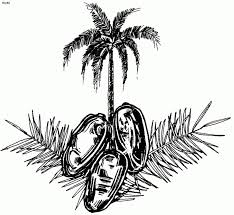
\includegraphics[scale=0.2]{Image/date.jpeg}\selectfont প্যাকেটজাত \selectlanguage{english} Dabbas, Neghal,
\includegraphics[scale=0.05]{Image/bee2.png} Lulu, Khalas \selectlanguage{bengali} ও\selectlanguage{english} Moriom \selectlanguage{bengali}খেজুর, শুকনা খেজুর; কালোজিরা, সরিষা ও  লিচু ফুলের মধু, সুন্দরবনের মধু; কালোজিরা ও তিলের তেল; কালোজিরা, কিসমিস, কাজুবাদাম, কাঠবাদাম  পাওয়া যায়\\}{\fontsize{36}{43.2}\selectfont \selectlanguage{english}01515-611989(Md. Al-Helal, CSE, MS)\\ \selectlanguage{bengali} রুম \selectlanguage{english}- 1406, \selectlanguage{english}Ex-1, \selectlanguage{bengali}শহীদুল্লাহ হল\\} {\fontsize{20}{24} \selectfont \selectlanguage{english} For free delivery order here \textbf{www.facebook.com/Honey\&Date}\\}\vspace{1.1cm}}
\end{document}
